
\section{Teoría general de grafos}


	En matemáticas, la \emph{teoría de grafos} estudia estructuras matemáticas usadas para modelar relaciones por pares entre objetos. 


\subsection{Definición de grafo}

{Concepto de gráfo}
	Un \emph{grafo} $G$ consiste de:
	\begin{enumerate}[(a)]
		\item Un conjunto $V$ cuyos elementos son llamados \emph{v\'ertices,} puntos o nodos de $G.$
		\item Un conjunto $E$ de pares (no ordenados) de distintos vertices, a los que llamaremos \emph{aristas} de $G.$
	\end{enumerate}
	
	Denotaremos un grafo por $G(V,E)$ cuando querramos enfatizar los componentes del mismo.



	\begin{rem}
		Debido a una ambig\"uedad en la traducción del ingl\'es al espa\~nol, en ocasiones, a un grafo tambi\'en se le conoce como \emph{gráfica,} que se puede confundir con el concepto de teoría de conjuntos. En este material, a veces utilizaremos \textit{gráfica,} pero debe entenderse como un grafo. 
	\end{rem}



	\begin{figure}[h!]
		\centering
		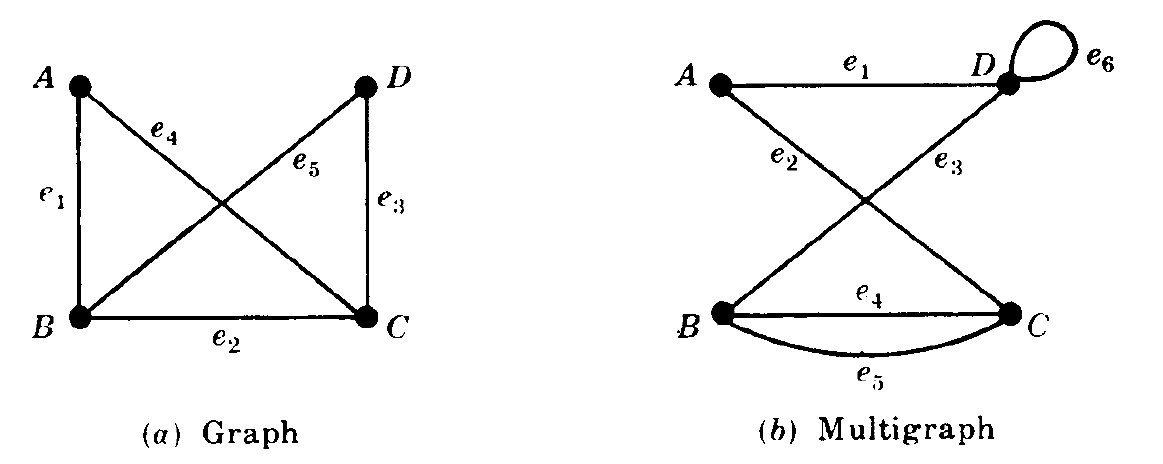
\includegraphics[width=12cm,keepaspectratio=true]{./md/grafos.png}
		% grafos.png: 0x0 pixel, 300dpi, 0.00x0.00 cm, bb=
		\caption{Grafos y multigrafos}
		\label{fig:md0501}
	\end{figure}
	


{Multigrafos}
	Consideremos la figura \ref{fig:md0501} (b). Las aristas $e_{4}$y $e_{5}$ son llamadas \emph{aristas multiples} ya que conectan los mismos extremos,  mientras que la arista $e_{6}$ es llamada \emph{bucle} ya que conecta un v\'ertice consigo mismo. 
	



	Tales diagramas son llamados \emph{multigrafos;}  la definición formal de grafo no admite aristas multiples ni bucles. 



	\begin{rem}
		Sin embargo, algunos textos utilizan ``grafos'' para referirse a lo que nosotros llamaremos multigrafos, mientras que ocupan ``grafo simple'' para lo que nosotros llamaremos grafos.
	\end{rem}
	


{Grado de un v\'ertice}
	El \emph{grado} de un v\'ertice $v$ es un grafo $G,$ denotado por $\deg(v),$ es igual al número de aristas in $G$ que contienen a $v,$ es decir, que \emph{inciden} en $v.$



	Dado que cada arista incide en dos v\'ertices diferentes, tenemos el siguiente resultado simple pero importante:
	\begin{thm}
		La suma de los grados de los v\'ertices en un grafo $G$ es el doble del número de aristas. 
	\end{thm}
	



	\begin{problema}
		En el grafo de la figura \ref{fig:md0501}(a), tenemos que 
		$$\deg(A)=2, \; \deg(B)=3,\; \deg(C)=3, \; \deg(D)=2.$$
		
		
		La suma de los grados es igual a 10, que es dos veces el número de aristas. 
	\end{problema}
	



	\begin{defn}
		Diremos que un v\'ertice es \emph{par} o \emph{impar} de acuerdo a la paridad de su grado. 
		
		En el ejemplo anterior, tanto $A$ com $D$ son v\'ertices pares, mientras que $B$ y $C$ son impares.
	\end{defn}
	



	\begin{rem}
		Diremos que un vertice de grado cero está \emph{aislado.}
	\end{rem}


{Gráfos finitos y triviales}
	Diremos que un grafo  es \emph{finito} si tiene un número finito de v\'ertices y un número finito de aristas. 
	
	Observe que un número finito de v\'ertices implica un número finito de aristas; pero no lo contrario no es necesariamente cierto. 
	
	Diremos que un grafo con un único v\'ertice, sin aristas,  es \emph{trivial.}\



	\begin{rem}
		A menos que se indique de otra manera, sólo trataremos con grafos finitos. 
	\end{rem}
	


\subsection{Subgrafos y grafos homeomorfos e isomorfos}


	Ahora, discutiremos relaciones de equivalencia entre grafos.


{Subgrafos}
	Consideremos un grafo $G(V,E).$ Diremos que otro grafo $H(V',E')$ es un \emph{subgrafo} de $G$ si los v\'ertices y aristas de $H$ están contenidos en los v\'ertices y aristas de $G,$ es decir, 
	$$
	V'\subset V, \; E' \subset E.
	$$



	En particular:
	\begin{enumerate}[(a)]
		\item Un subgrafo $H(V',E')$ de $G(V,E)$ es llamado subgrafo \emph{inducido} por sus v\'ertices $V'$ si el conjunto de aristas $E'$ contiene todas las aristas en $G$ cuyo extremos pertenecen a los v\'ertices en $H.$ 
		\item Si $v$ es un v\'ertice en $G,$ entonces \emph{$G-v$} es el subgrafo de $G$ ontenido al borrar $v$ de $G$ y todas las aristas en $G$ que inciden en $v.$ 
		\item Si $e$ es una arista en $G,$ entonces \emph{$G-e$} es el subgrafo de $G$ obtenido borrando la arista $e$ en $G.$
	\end{enumerate}
	


{Grafos isomorfos}
	Dos grafos $G(V,E)$ y $G^{*}(V^{*},E^{*})$ son llamados \emph{isomorfos} si existe una función biyectiva $f: V \to V^{*}$ tal que: $\set{u,v}$ es una arista de $G$ si y solo si $\set{f(u),f(v)}$ es una arista de $G^{*}.$
	 
	
	La idea es que estos grafos son equivalentes, aún cuando sus representaciones pueden lucir muy diferentes.



	\begin{figure}[h!]
		\centering
		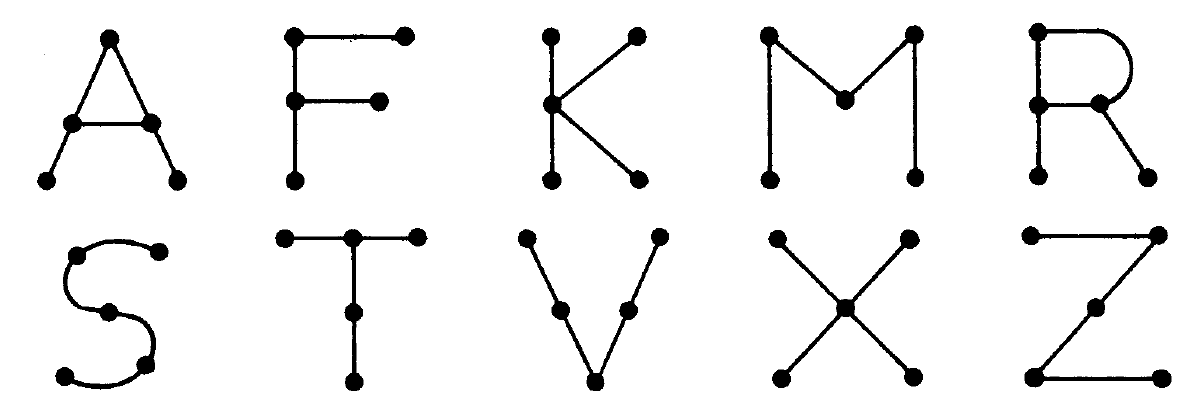
\includegraphics[width=10cm,keepaspectratio=true]{./md/letras.png}
		% letras.png: 0x0 pixel, 300dpi, 0.00x0.00 cm, bb=
		\caption{Grafos isomorfos.}
		\label{fig:md0502}
	\end{figure}
	


{Grafos homeomorfos}
	Dado un grafo $G,$ podemos obtener un nuevo grafo dividiendo una arista de $G$ con v\'ertices adicionales. 
	
	Dos grafos $G$ y $G^{*}$ son llamados \emph{homeomorfos} si pueden obtenerse de gráficas isomorfas a trav\'es de este m\'etodo. 



	\begin{figure}[h!]
		\centering
		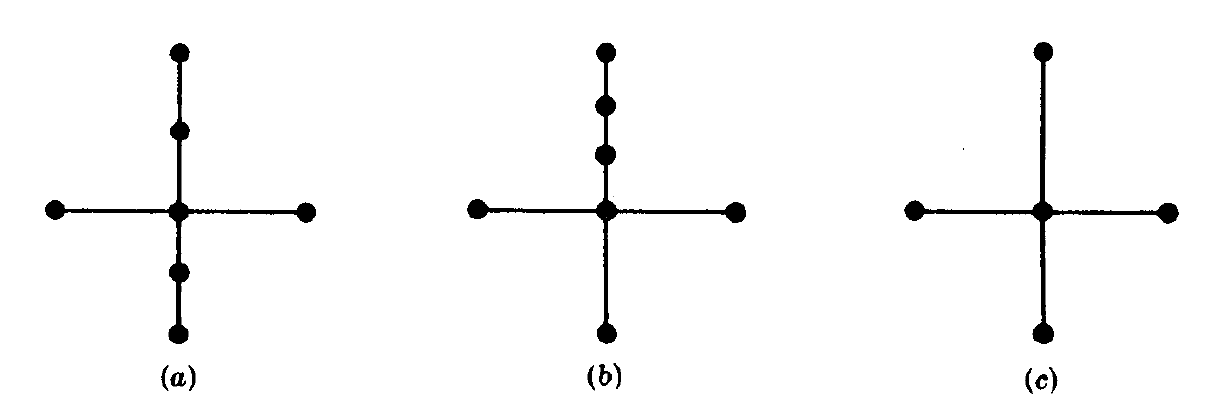
\includegraphics[width=8cm,keepaspectratio=true]{./md/homomorfas.png}
		% homomorfas.png: 0x0 pixel, 300dpi, 0.00x0.00 cm, bb=
		\caption{Grafos homomorfos}
		\label{fig:md0503}
	\end{figure}
	
	Los grafos $(a)$ y $(b)$ son homeomorfos, ya que se pueden obtener a\~nadiendo v\'ertices al grafo $(c).$


\subsection{Caminos y conexidad}


	Un \emph{camino} en un (multi)grafo $G$ consiste en una sucesión alternante de v\'ertices y arista de la forma
	$$
	v_{0}, e_{1}, v_{1}, ..., e_{n-1}, v_{n-1}, e_{n}, v_{n}
	$$
	donde cada arista $e_{i}$ contiene los v\'ertices $v_{i-1}$ y $v_{i}.$



	\begin{rem}
		Observe que en grafo, podemos simplificar la notación para un camino, indicando sólo los v\'ertices que recorre:
		$$v_{0}, v_{1},..., v_{n}.$$ 
	\end{rem}



	Diremos que el camino es \emph{cerrado} si $v_{n}=v_{0}.$ En otro caso, diremos que el camino conecta $v_{0}$ con $v_{n}.$
	 
	
	Un \emph{camino simple} es aquel en el cual todos los v\'ertices son distintos. Mientras que un camino en el que todas las aristas son distintas se llama \emph{paseo}.
	



	La \emph{longitud} de un camino es igual a número de aristas en la sucesión que lo define.
	 



	Un \emph{ciclo} es un camino cerrado de \emph{longitud} al menos 3, en el que todos los v\'ertices son distintos, excepto el inicial $v_{0}$ y el final $v_{n}.$
	
	
	Un ciclo de longitud $k$ es llamado \emph{$k-$ciclo.}



	\begin{figure}[h!]
		\centering
		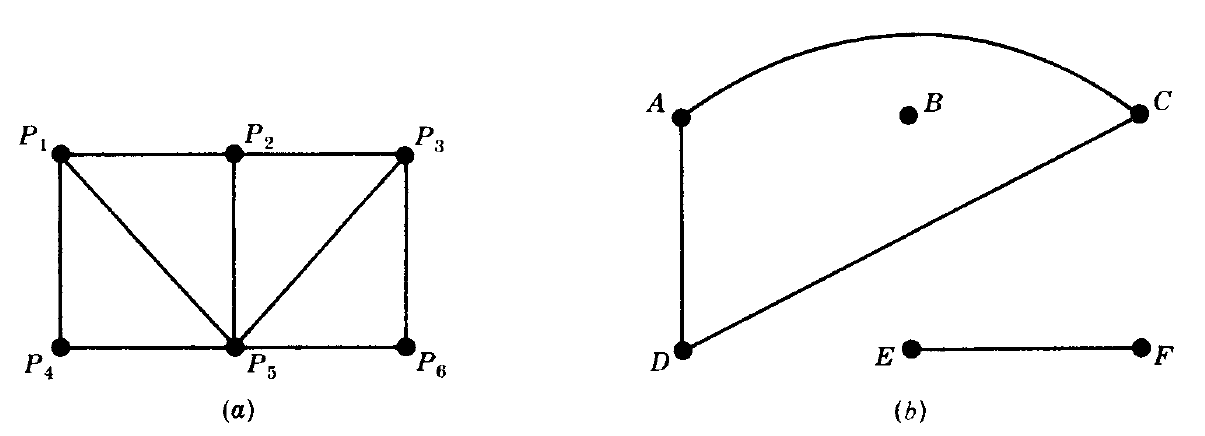
\includegraphics[width=10 cm,keepaspectratio=true]{./md/grafo_8_8.png}
		% grafo_8.8.png: 0x0 pixel, 300dpi, 0.00x0.00 cm, bb=
		\caption{Conexidad en grafos}
		\label{fig:md0504}
	\end{figure}



	\begin{problema}
		\label{lip:exmp:8.1}
		Consideremos el grafo \ref{fig:md0504}(a). Considere las siguientes sucesiones
		\begin{align*}
			\a&=\left( P_{4}, P_{1}, P_{2}, P_{5}, P_{1},P_{2}, P_{3}, P_{6}  \right), \\
			\b&=\left( P_{4}, P_{1}, P_{5}, P_{2}, P_{6} \right) \\
			\gam&= \left( P_{4}, P_{1}, P_{5}, P_{2}, P_{3}, P_{5}, P_{6} \right)\\
			\del&=\left( P_{4}, P_{1}, P_{5}, P_{3}, P_{6} \right).
		\end{align*}
		
	\end{problema}
	



	\begin{figure}[h!]
		\centering
		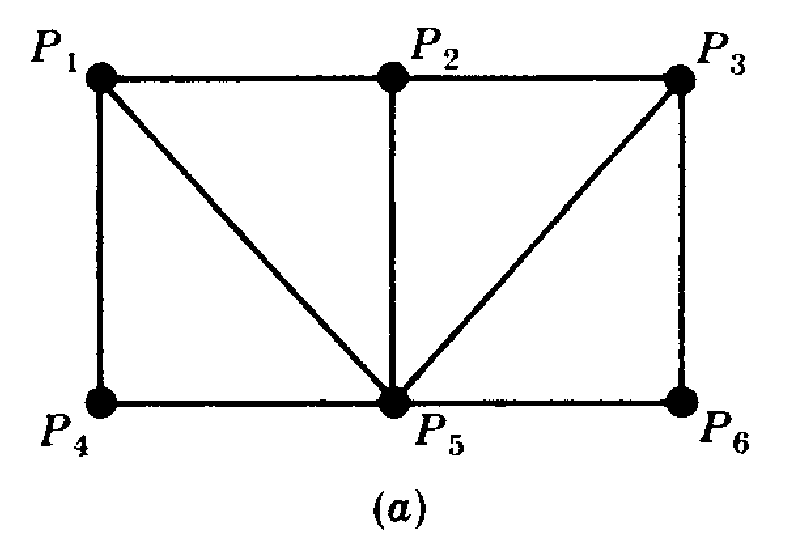
\includegraphics[width=5cm,keepaspectratio=true]{./md/grafo_8_8_a.png}
		% grafo_8_8_a.png: 0x0 pixel, 300dpi, 0.00x0.00 cm, bb=
	\end{figure}
	$\a$ es un camino de $P_{4}$ a $P_{6},$ pero no es un paseo.



	\begin{figure}[h!]
		\centering
		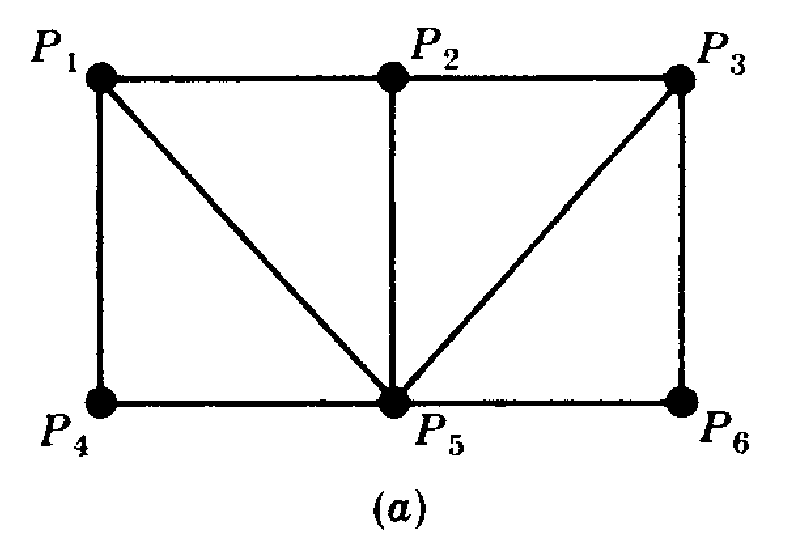
\includegraphics[width=5cm,keepaspectratio=true]{./md/grafo_8_8_a.png}
		% grafo_8_8_a.png: 0x0 pixel, 300dpi, 0.00x0.00 cm, bb=
	\end{figure}
	$\b$ no es un camino, ya que no existe alguna arista $\set{P_{2}, P_{6}}.$



	\begin{figure}[h!]
		\centering
		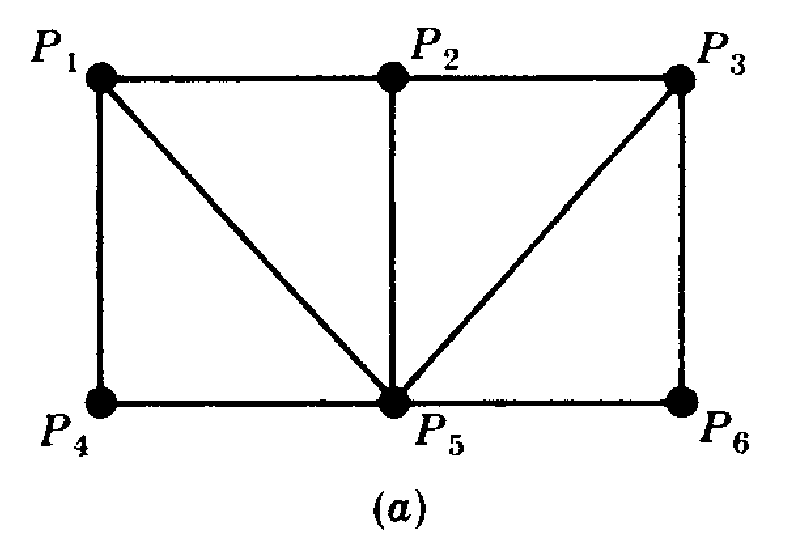
\includegraphics[width=5cm,keepaspectratio=true]{./md/grafo_8_8_a.png}
		% grafo_8_8_a.png: 0x0 pixel, 300dpi, 0.00x0.00 cm, bb=
	\end{figure}
	$\gam$ es un paseo, pero no es un camino simple.



	\begin{figure}[h!]
		\centering
		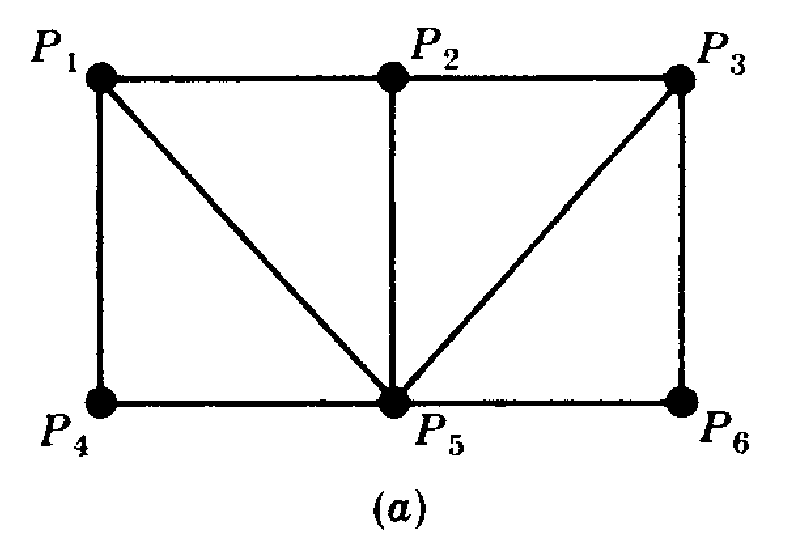
\includegraphics[width=5cm,keepaspectratio=true]{./md/grafo_8_8_a.png}
		% grafo_8_8_a.png: 0x0 pixel, 300dpi, 0.00x0.00 cm, bb=
	\end{figure}
	$\del$ es un camino simple de $P_{4}$ a $P_{6},$ pero no es el camino más corto, es decir, con el meno número de aristas. ?`Cuál es el camino más corto?



	Eliminando aristas innecesarias, no es difícil ver que cualquier camino de $u$ a $v$ puede ser reemplazado por un camino simple.
	 
	
	Formalmente:
	\begin{thm}
		Existe un camino del v\'ertice $u$ a $v$ si y solo si existe un camino simple de $u$ a $v.$
	\end{thm}
	


{Conexidad y componentes conexas}
	Un grafo $G$ es conexo si existe un camino entre cualesquiera dos v\'ertices.  Por ejemplo, el grafo \ref{fig:md0504}(a) es conexo, pero no así el grafo \ref{fig:md0504}(b).
	\begin{figure}[h!]
		\centering
		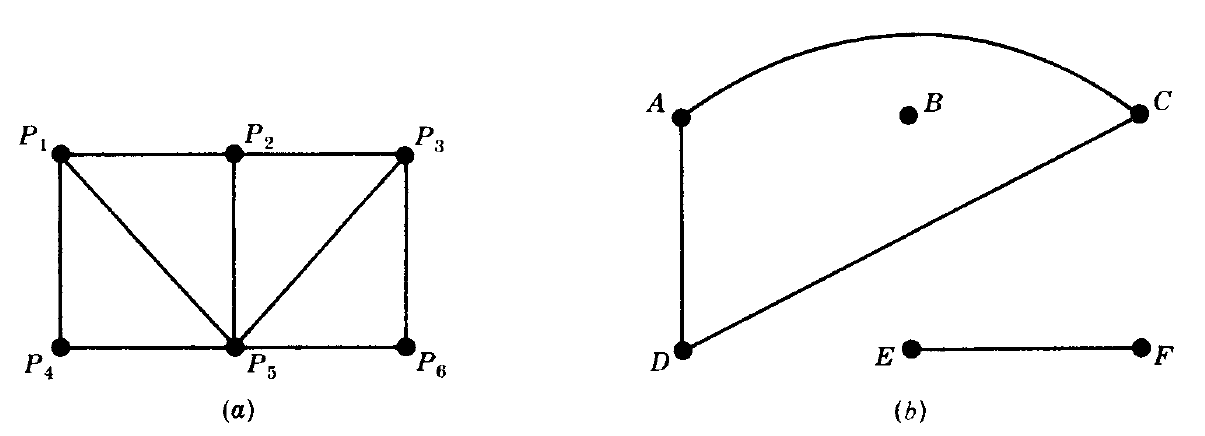
\includegraphics[width=8cm,keepaspectratio=true]{./md/grafo_8_8.png}
		% grafo_8_8.png: 0x0 pixel, 300dpi, 0.00x0.00 cm, bb=
	\end{figure}
	



	Consideremos un grafo $G.$ Un subgrafo conexo $H$ de $G$ es llamado \emph{componente conexa} de $G$ si $H$ no está contenido de manera propia en cualquier otro grafo conexo de $G.$ 
	
	Por ejemplo, el grafo \ref{fig:md0504}(b) tiene tres componentes conexas.
	
	\begin{figure}[h!]
		\centering
		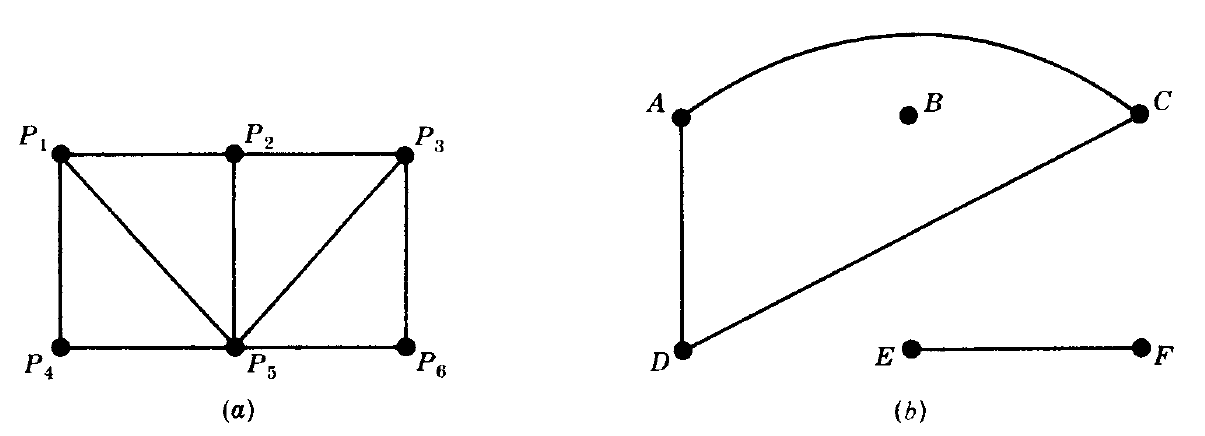
\includegraphics[width=8cm,keepaspectratio=true]{./md/grafo_8_8.png}
		% grafo_8_8_a.png: 0x0 pixel, 300dpi, 0.00x0.00 cm, bb=
	\end{figure}
	



	\begin{rem}
		Formalmente, permitiendo que un v\'ertice $u$ est\'e conectado consigo mismo, la relación \begin{center}
			\texttt{$u$ está conectado con $v$}                                                                                                                                                                                            \end{center}
		es una relación de equivalencia en el conjunto de v\'ertices del grafo $G,$  y las clases de equivalencia de esta relación son las componentes conexas de $G.$
	\end{rem}
	


{Distancia y diametro}
	Consideremos un grafo conexo $G.$ La distancia entre  dos v\'ertices $u$ y $v$ en $G,$ denotada por $d(u,v),$ es la longitud del camino más corto entre $u$ y $v.$ E\~n diametro de $G,$ escrito $diam(G),$ es la distancia máxima entre cualesquiera dos puntos en $G.$ 



	\begin{figure}[h!]
		\centering
		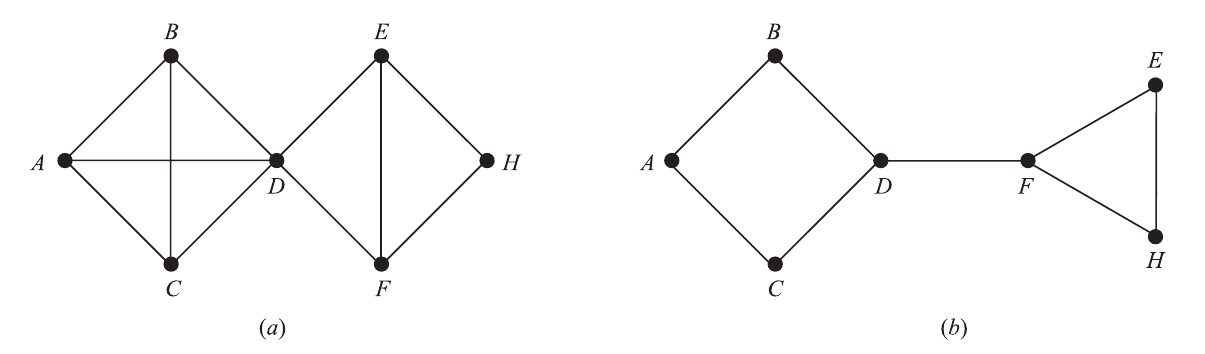
\includegraphics[width=10cm,keepaspectratio=true]{./md/grafo_8_9.png}
		% grafo_8_9.png: 0x0 pixel, 300dpi, 0.00x0.00 cm, bb=
		\caption{Distancia y diametro}
		\label{fig:md0505}
	\end{figure}
	Por ejemplo, en el grafo \ref{fig:md0505}(a), el diamtero es $3,$ mientras que en el (b), el diametro es 4.


{Puntos de corte y puentes}
	Sea $G$ un grafo conexo. Un v\'ertice $v$ en $G$ es llamado \emph{punto de corte} si $G-v$ es disconexo. Una arista $e$ en $G$ es llamada \emph{puente} si $G-e$ es disconexo. 
	
	\begin{figure}[h]
		\centering
		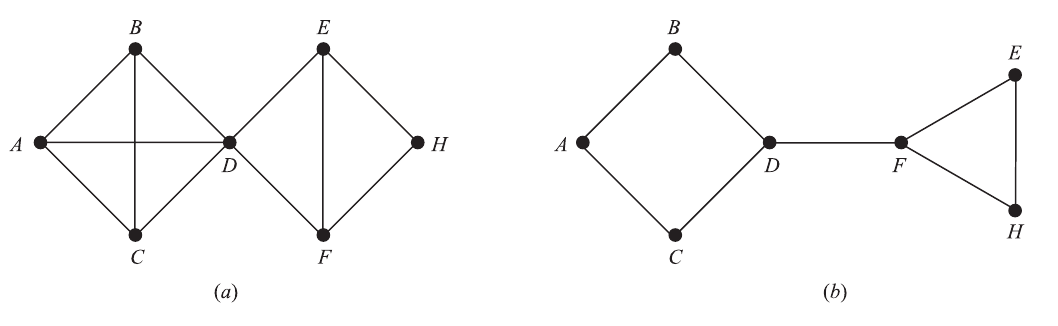
\includegraphics[height=3cm,keepaspectratio=true]{./md/fig0809.png}
		% fig0809.png: 0x0 pixel, 300dpi, 0.00x0.00 cm, bb=
		\caption{Puntos de corte y puentes}
		\label{fig:0809}
	\end{figure}
	


\subsection{Grafos transitables y eulerianos}

	\begin{figure}[h!]
		\centering
		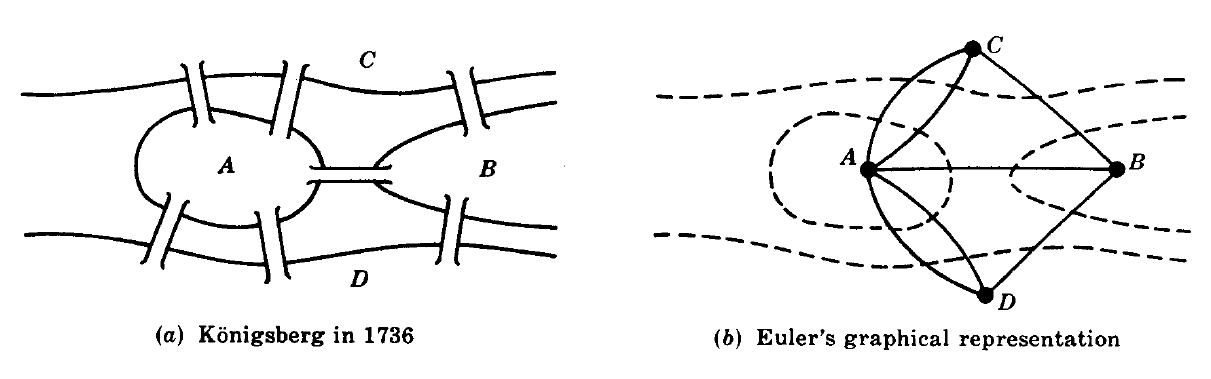
\includegraphics[width=10cm,keepaspectratio=true]{./md/grafo_8_10.png}
		% grafo_8_10.png: 0x0 pixel, 300dpi, 0.00x0.00 cm, bb=
		\caption{Puentes de K\"onigsberg y su representación}
		\label{fig:md0506}
	\end{figure}



	Un multigrafo es llamado \emph{transitable} si existe un \emph{paseo} (un camino dónde todos las aristas son diferentes), que incluye \emph{todos los v\'ertices y todas las aristas.}
	
	Tal paseo será llamado  \emph{paseo transitable}. 
	
	
	\begin{rem}
		De manera equivalente, un paseo transitable es un camino en el que todos los v\'ertices se transitan \emph{al menos} una vez,  pero las aristas \emph{exactamente} una vez.
	\end{rem}
	



	
	\begin{prop}
		Cualquier grafo conexo y finito con exactamente dos v\'ertices impares es transitable. Un paseo transitable puede comenzar en alguno de los v\'ertices impares y terminar en el otro v\'ertice impar.
	\end{prop}



	Un grafo $G$ es llamado \emph{grafo Euleriano} si existe un \emph{paseo transitable cerrado}.
	
	
	A tal paseo le llamaremos \emph{paseo Euleriano.}
	
	
	\begin{thm}[Euler]
		Un grafo conexo y finito es Euleriano si y solo si cada v\'ertice tiene grado par. 
	\end{thm}
	


{Grafos hamiltonianos}
	En la definición de grafos Eulerianos se enfatizó pasar por todas las aristas. 
	
	
	Ahora, nos enfocaremos en visitar todos los v\'ertices. 



	Un \emph{circuito Hamiltoniano} es un grafo $G$ es un camino cerrado que visita cada v\'ertice en $G$ \emph{exactamente} una vez.
	
	
	Si $G$ admite un circuito Hamiltoniano, entonces $G$ es llamado un \emph{grafo Hamiltoniano.}
	
	
	\begin{rem}
		En la definición de circuito Hamiltoniano, cuando decimos que el camino \emph{visita} cada v\'ertice exactamente una vez significa que, aunque el v\'ertice inicial tiene que ser el mismo que el final, todos los demás v\'ertices intermedios deben ser distintos.
	\end{rem}
	



	\begin{rem}
		Un {\color{red}paseo Euleriano} atraviesa {\color{red}cada una de las aristas} exactamente una vez, pero los v\'ertices se pueden repetir, mientras que un {\color{blue}circuito Hamiltoniano} visita {\color{blue}cada uno de los v\'ertices} exactamente una vez, pero las aristas pueden repetirse. 
		
		
	\end{rem}
	
	
	
	\begin{thm}
		Sea $G$ un grafo conexo con $n$ v\'ertices. Entonces $G$ es Hamiltoniano si $n\geq 3$ y $n \leq \deg(v)$ para cada v\'ertice $v$ en $G.$
	\end{thm}
	



	\begin{figure}[h!]
		\centering
		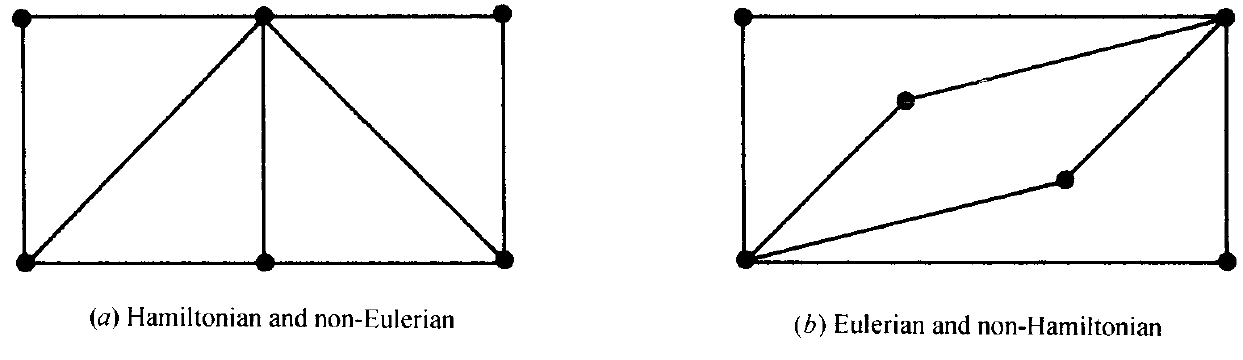
\includegraphics[width=10 cm]{./md/grafo_8_11.png}
		% grafo_8_11.png: 0x0 pixel, 300dpi, 0.00x0.00 cm, bb=
		\caption{Circuitos Eulerianos y Hamiltonianos}
		\label{fig:md 0506}
	\end{figure}
	



\subsection{Matriz de adyacencia}


	Supongamos que $G$ es un gráfo con $m$ v\'ertices y que estos han sido ordenados:
	$$
	v_{1}, v_{2},...,v_{m}.
	$$
	
	Entonces, la \emph{matriz de adyacencia} $A=\left( a_{i,j} \right)$ del grafo $G$ es la matriz de dimensión $m\times m$ definida por:
	$$a_{i,j}=
	\begin{cases}
		1 & v_{i}\texttt{ es adyacente a }v_{j}\\
		0 & \texttt{en otro caso}
	\end{cases}
	$$



	\begin{figure}[h]
		\centering
		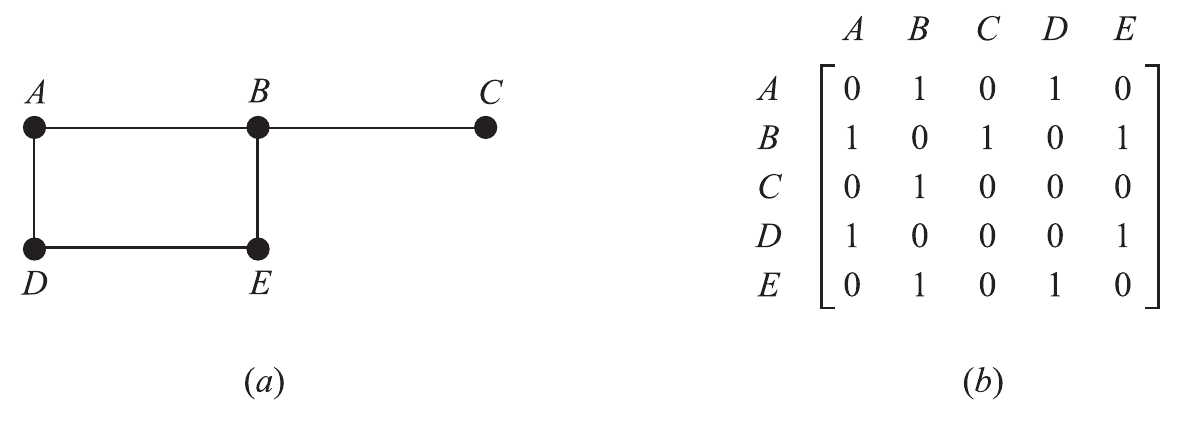
\includegraphics[width=10cm,keepaspectratio=true]{./md/fig0827.png}
		% fig0827.png: 0x0 pixel, 300dpi, 0.00x0.00 cm, bb=
		\caption{Matriz de adyacencia}
		\label{fig:0827}
	\end{figure}
	


